\documentclass{beamer} %

%%%BASICS
\usepackage{fontspec}
%\usepackage[utf8]{inputenc}
\usepackage{csquotes}
\usepackage{pdfpages}

%%%START THEME SETTINGS
\usetheme{Dresden}
\usecolortheme{beaver}
\usefonttheme{professionalfonts}
\setbeamertemplate{itemize item}{\color{red}$\blacksquare$}
%%%END THEME SETTINGS

%%%START APA
%\usepackage[british]{babel}
%\usepackage[backend=biber,style=apa]{biblatex}
%\DeclareLanguageMapping{british}{british-apa}
%\addbibresource{references.bib}
%% APA citing
%% \cite{t} - Uthor und Richter, 2010
%% \textcite{t} - Uthor und Riter (2010)
%% \parencite{t} - (Uthor & Riter, 2010)
%% \parencite[Chapt.~4]{t} - (Uthor & Riter, 2010, S. 15)
%%%END APA


\title[PSY 242 Developmental Psychology]{Genetic Expression}
\institute[College of Staten Island]{College of Staten Island, CUNY}
\author{Xiaomeng Ma}

\date{6th September 2018}

\begin{document} 
\begin{frame}
	\titlepage
\end{frame}
%------------------------------------------------------
\begin{frame}{Introduction}
\textbf{Nature VS Nurture?}
\pause
\begin{itemize}
    \item Francis Galton: Hereditary Genius (1869) and English Men of Science: Their Nature and Nurture (1874) 
    \\ studied case of “emniment men” and believed intelligence are is inherited
    \item John Stuart Mill, a philosopher, whose father is James Mill an economist, believed that men rose to eminence more because of family 
\end{itemize}
\end{frame}
%------------------------------------------------------
\begin{frame}{Modern Understanding of Heredity}
\begin{itemize}
    \item Gregor Mendel's pea garden
    \\ https://www.youtube.com/watch?v=Mehz7tCxjSE&vl=en
    \begin{figure}
        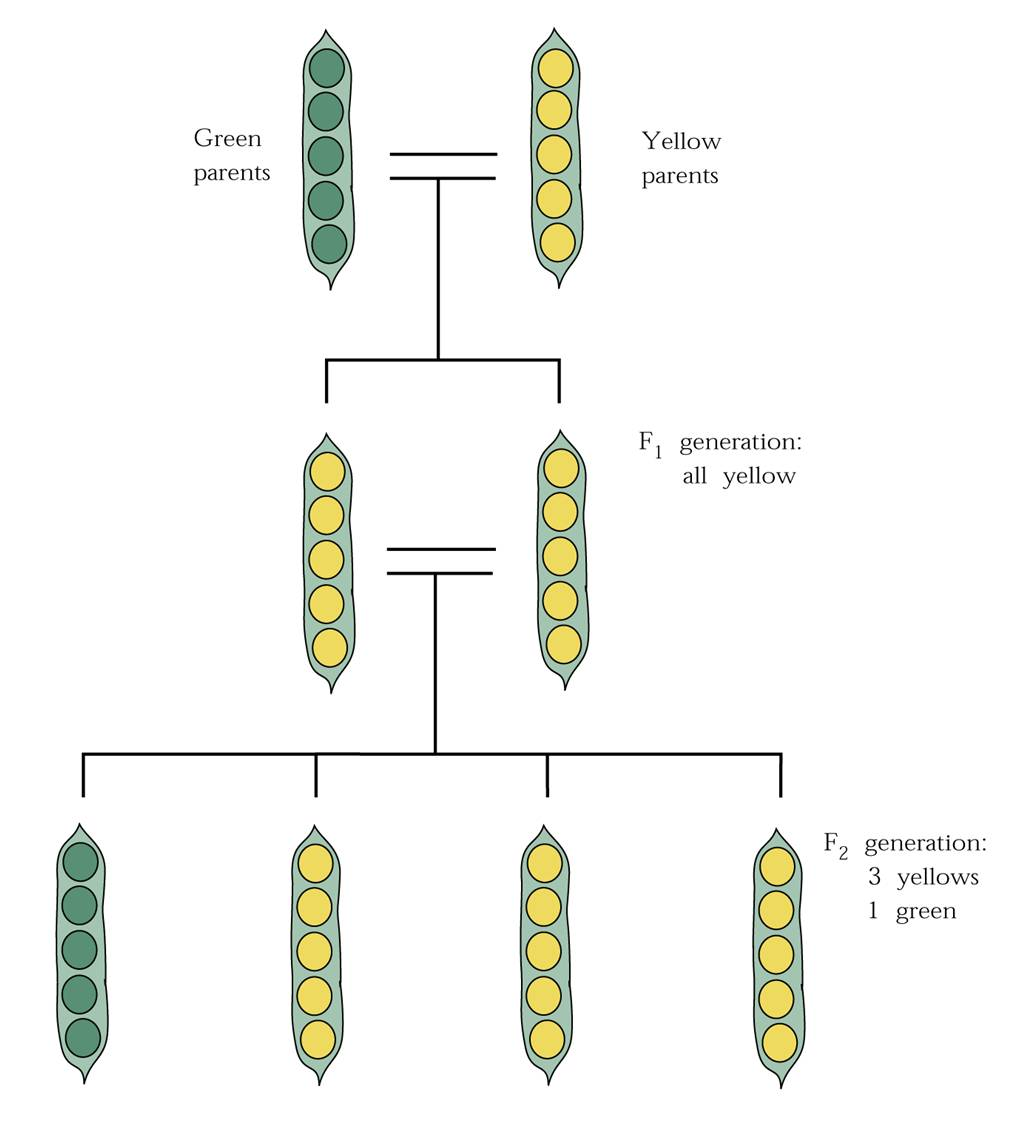
\includegraphics[width=\linewidth, height = 4cm]{MendelPeas.jpg}
    \end{figure}
\end{itemize}
\end{frame}
%------------------------------------------------------
\begin{frame}{Conception}
\begin{enumerate}
    \item <1-8> Gametes meet (sperm and egg meet) --- Fertilization
    \only <2> {https://www.youtube.com/watch?v=DGyRD9HnXVs}
    \item <3-8> Sperm and Egg combine --- Meiosis
    \only <4> {https://www.youtube.com/watch?v=lH9loPdk_nQ}
    \only <5> {\begin{figure}
        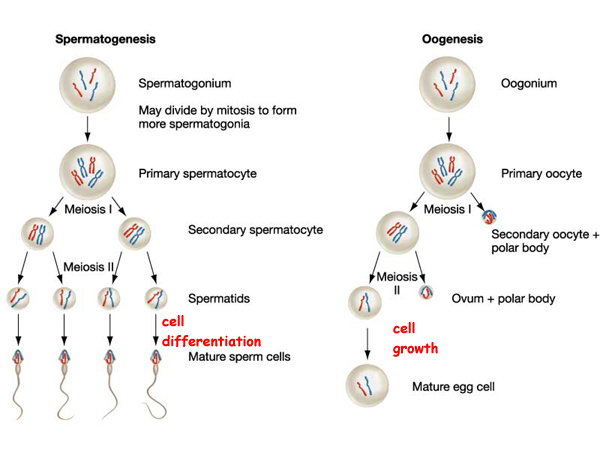
\includegraphics[width=15cm,
  height=6cm,
  keepaspectratio]{sf45x3.jpg}
    \end{figure}}
    \item <6-8> Fertilized Egg complete --- Zygote
    \only <7> {\begin{figure}
        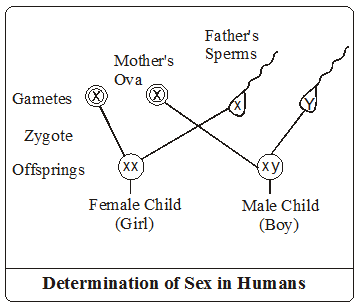
\includegraphics[width=15cm, height=4cm, keepaspectratio]{29330512035_8ac440754f_o.png}
    \end{figure}}
\end{enumerate}
\only<8>{\begin{itemize}
    \item \textbf{Germinal Development}: From Conception to 2 weeks
\end{itemize}}
\end{frame}
%------------------------------------------------------
\begin{frame}{Developmental Process}
\textcolor{red}{\textbf{Zygote - Embryo - Fetus}}
\begin{figure}
    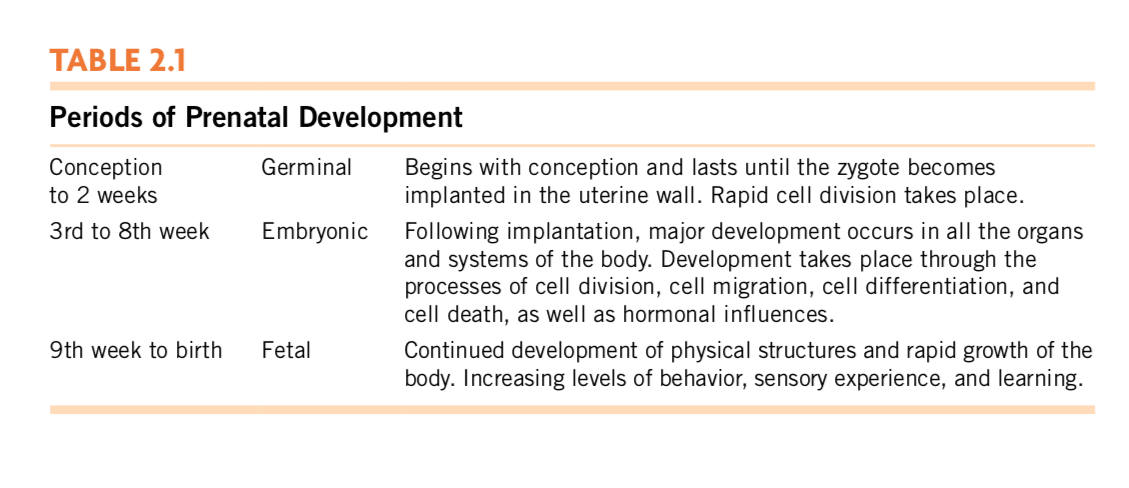
\includegraphics[width=\textwidth, height=8cm, keepaspectratio]{1.png}
\end{figure}
\end{frame}
%------------------------------------------------------
\begin{frame}{Zygote - Embryo -  Fetus}
\only<1>{https://www.youtube.com/watch?v=bHYAMjwgeV8}
\begin{itemize}
    \only<2,14>{\begin{itemize}
        \item Zygote: a fertilized egg cell
        \item Embryo: developing organism from the 3rd to 8th week of prenatal development
        \item Fetus: developing organism from the 9th week to birth
    \end{itemize}}
    \only<3-5,14>{\item Cell division (copy itself) --- Mitosis}
    \only<4>{\\https://www.youtube.com/watch?v=DwAFZb8juMQ}
    \only<5>{\begin{figure}
        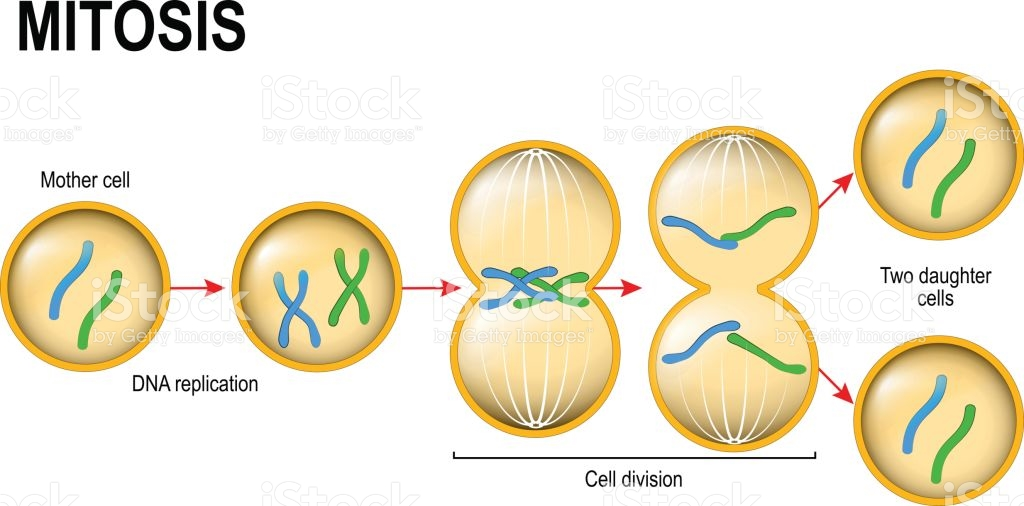
\includegraphics[width=\textwidth, height=6cm, keepaspectratio]{687251074.jpg}
    \end{figure}}
    \only<6-8,14> {\item Cell migration: newly formed cells move away from their originated point}
    \only<7>{\\https://www.youtube.com/watch?v=RQ6vkDr_Dec}
    \only<8>{\begin{figure}
        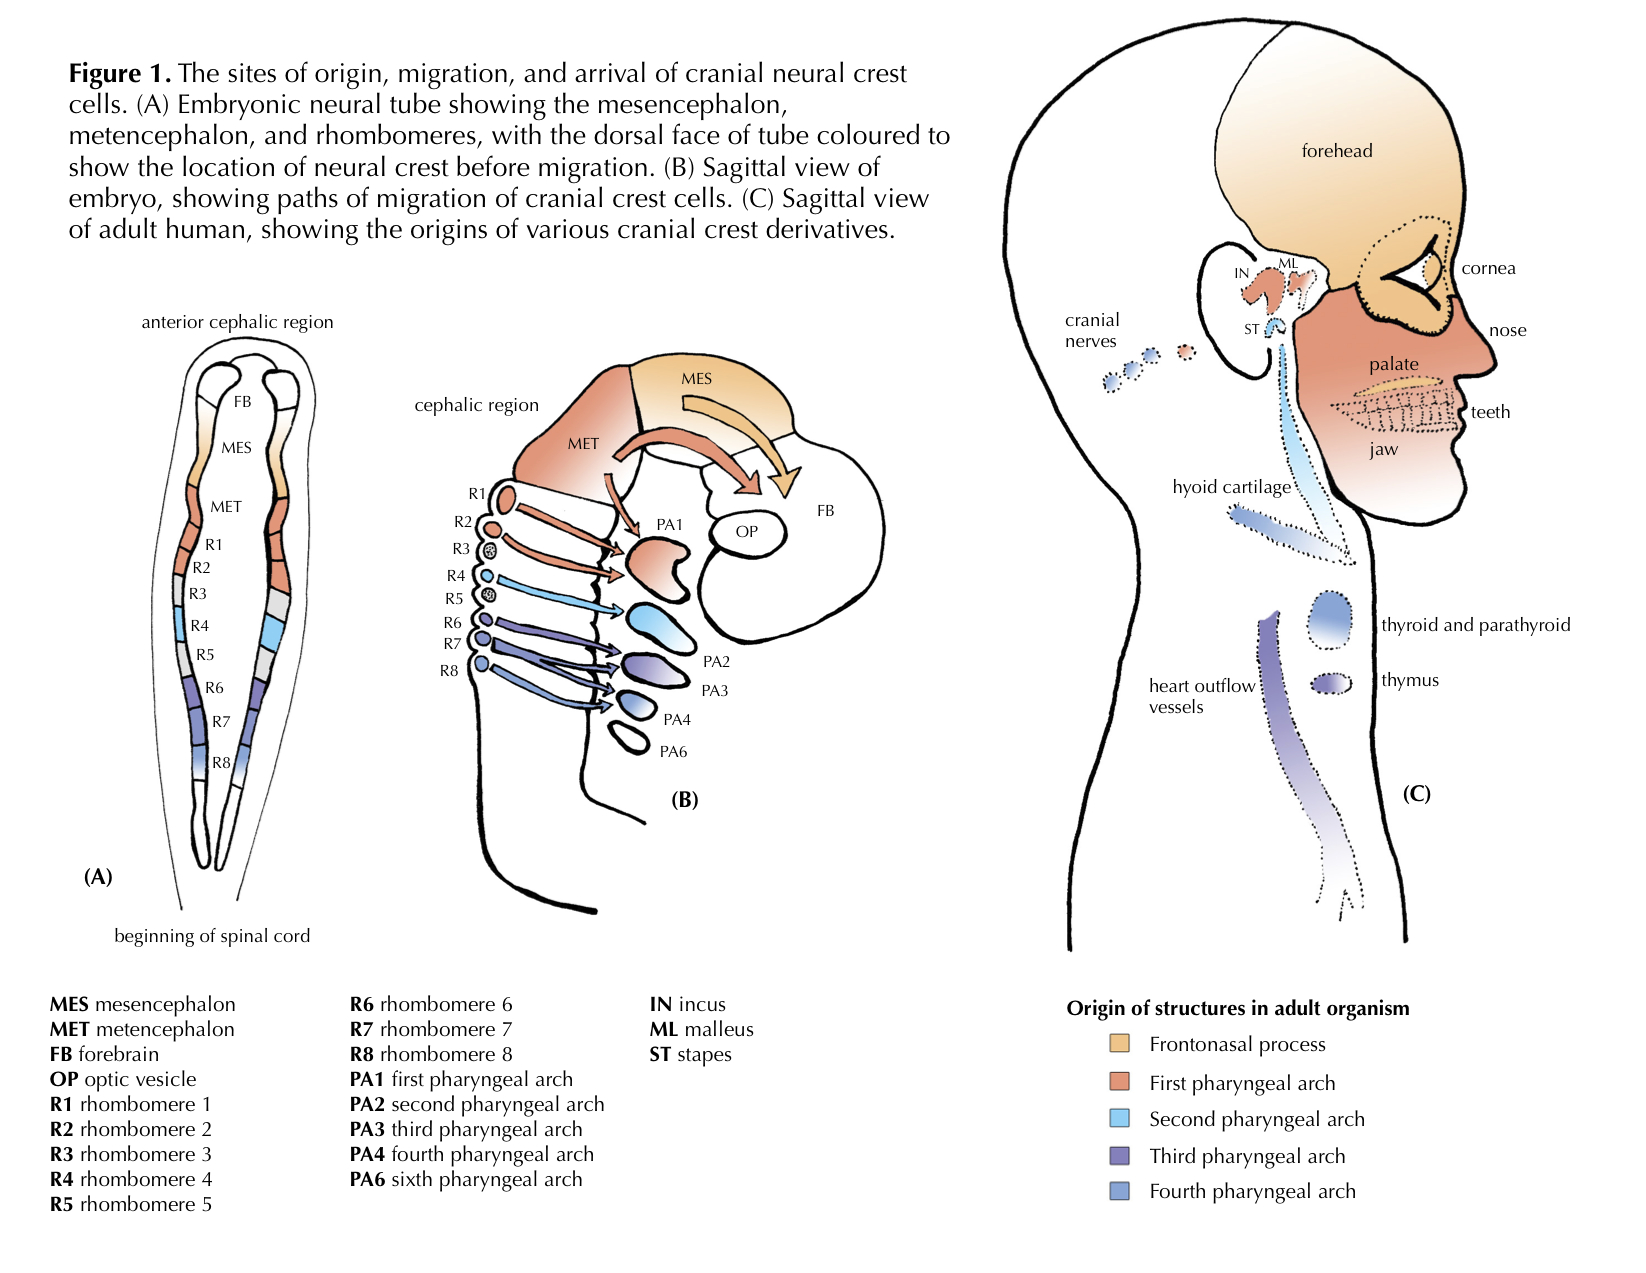
\includegraphics[width=\textwidth, height=6cm, keepaspectratio]{Cranial_Neural_Crest_Cells_-_migration.jpg}
    \end{figure}}
    \only<9-11,14> {\item Cell differentiation: embryonic stem cells grow into cells with specific functions}
    \only<10>{\begin{figure}
        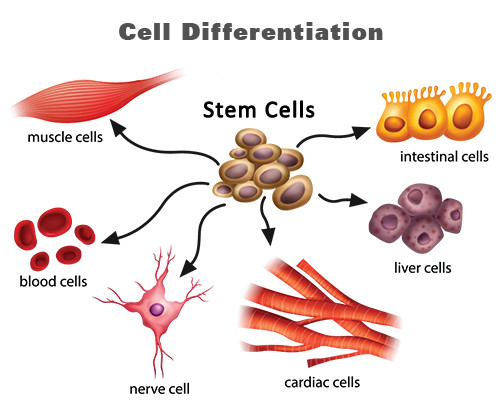
\includegraphics[width=\textwidth, height=6cm, keepaspectratio]{cell-differentiation.jpg}
            \end{figure}}
    \only<11>{\begin{itemize}
        \item Melynation
        \item Localization
    \end{itemize}}
    \only <12-14>{\item Apoptosis: cell suicide (e.g formation of fingers)}
    \only<13>{\begin{figure}
        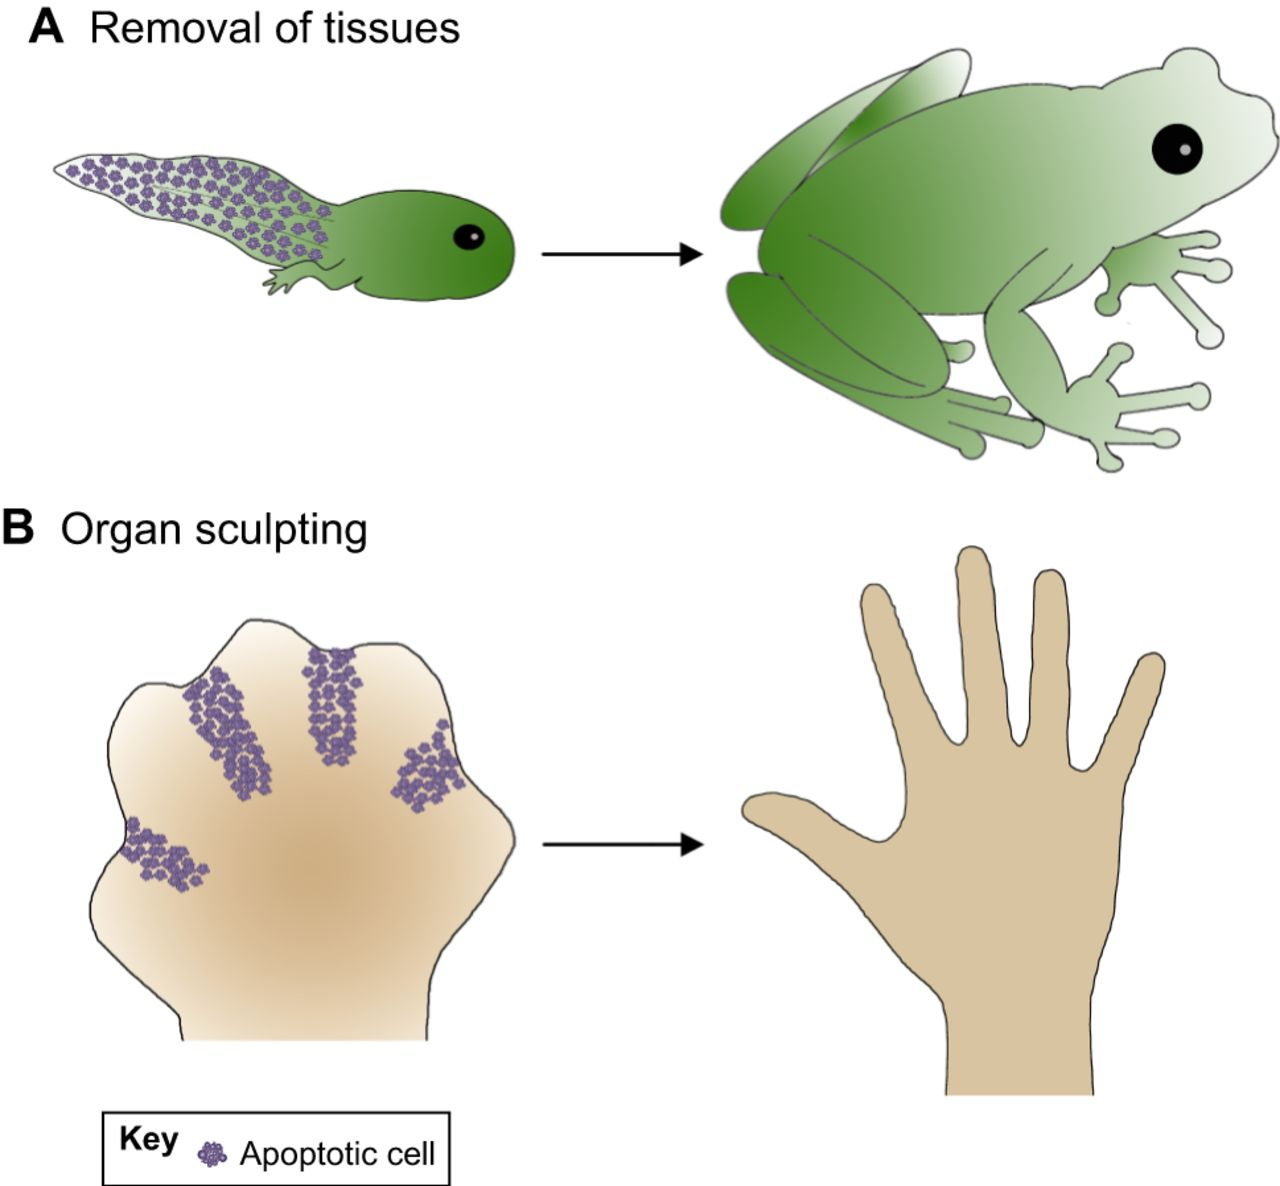
\includegraphics[width=\textwidth,height=6cm,keepaspectration]{F1.large.jpg}
    \end{figure}}
\end{itemize}
\end{frame}
%------------------------------------------------------
\begin{frame}{Early Development}
\begin{itemize}
    \item 4th day of conception: Development of Inner Mass Cells (when twins start to develop)
    \begin{figure}
        \centering
        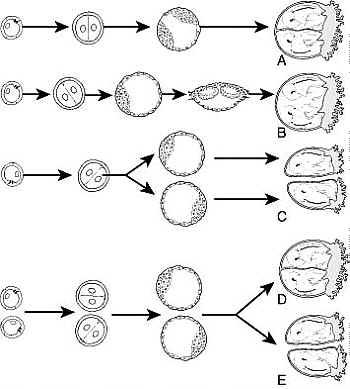
\includegraphics[width=\textwidth,height=6cm]{twindevelopment.jpg}
    \end{figure}
\end{itemize}
\end{frame}
%------------------------------------------------------
\begin{frame}{Early Development}
\begin{itemize}
    \item Day 7: Implantation (embryo enters uterus)
    \only<2>{\begin{figure}
        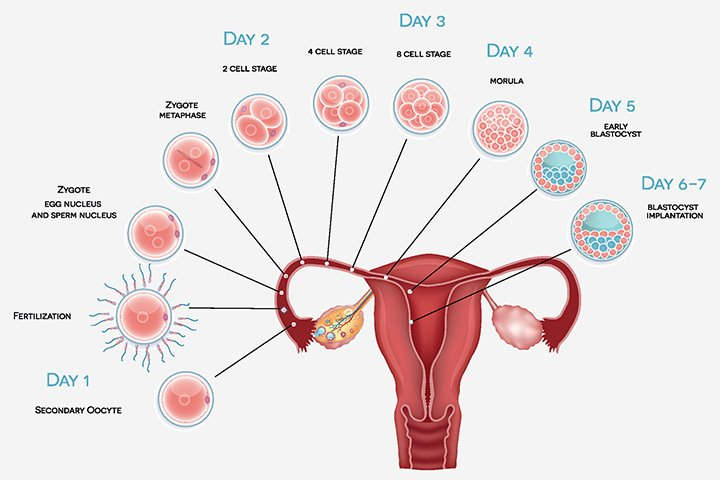
\includegraphics[width=\textwidth,height=6cm]{Pregnancy-Implantation.jpg}
    \end{figure}}
    \only<3>{\begin{figure}
        \centering
        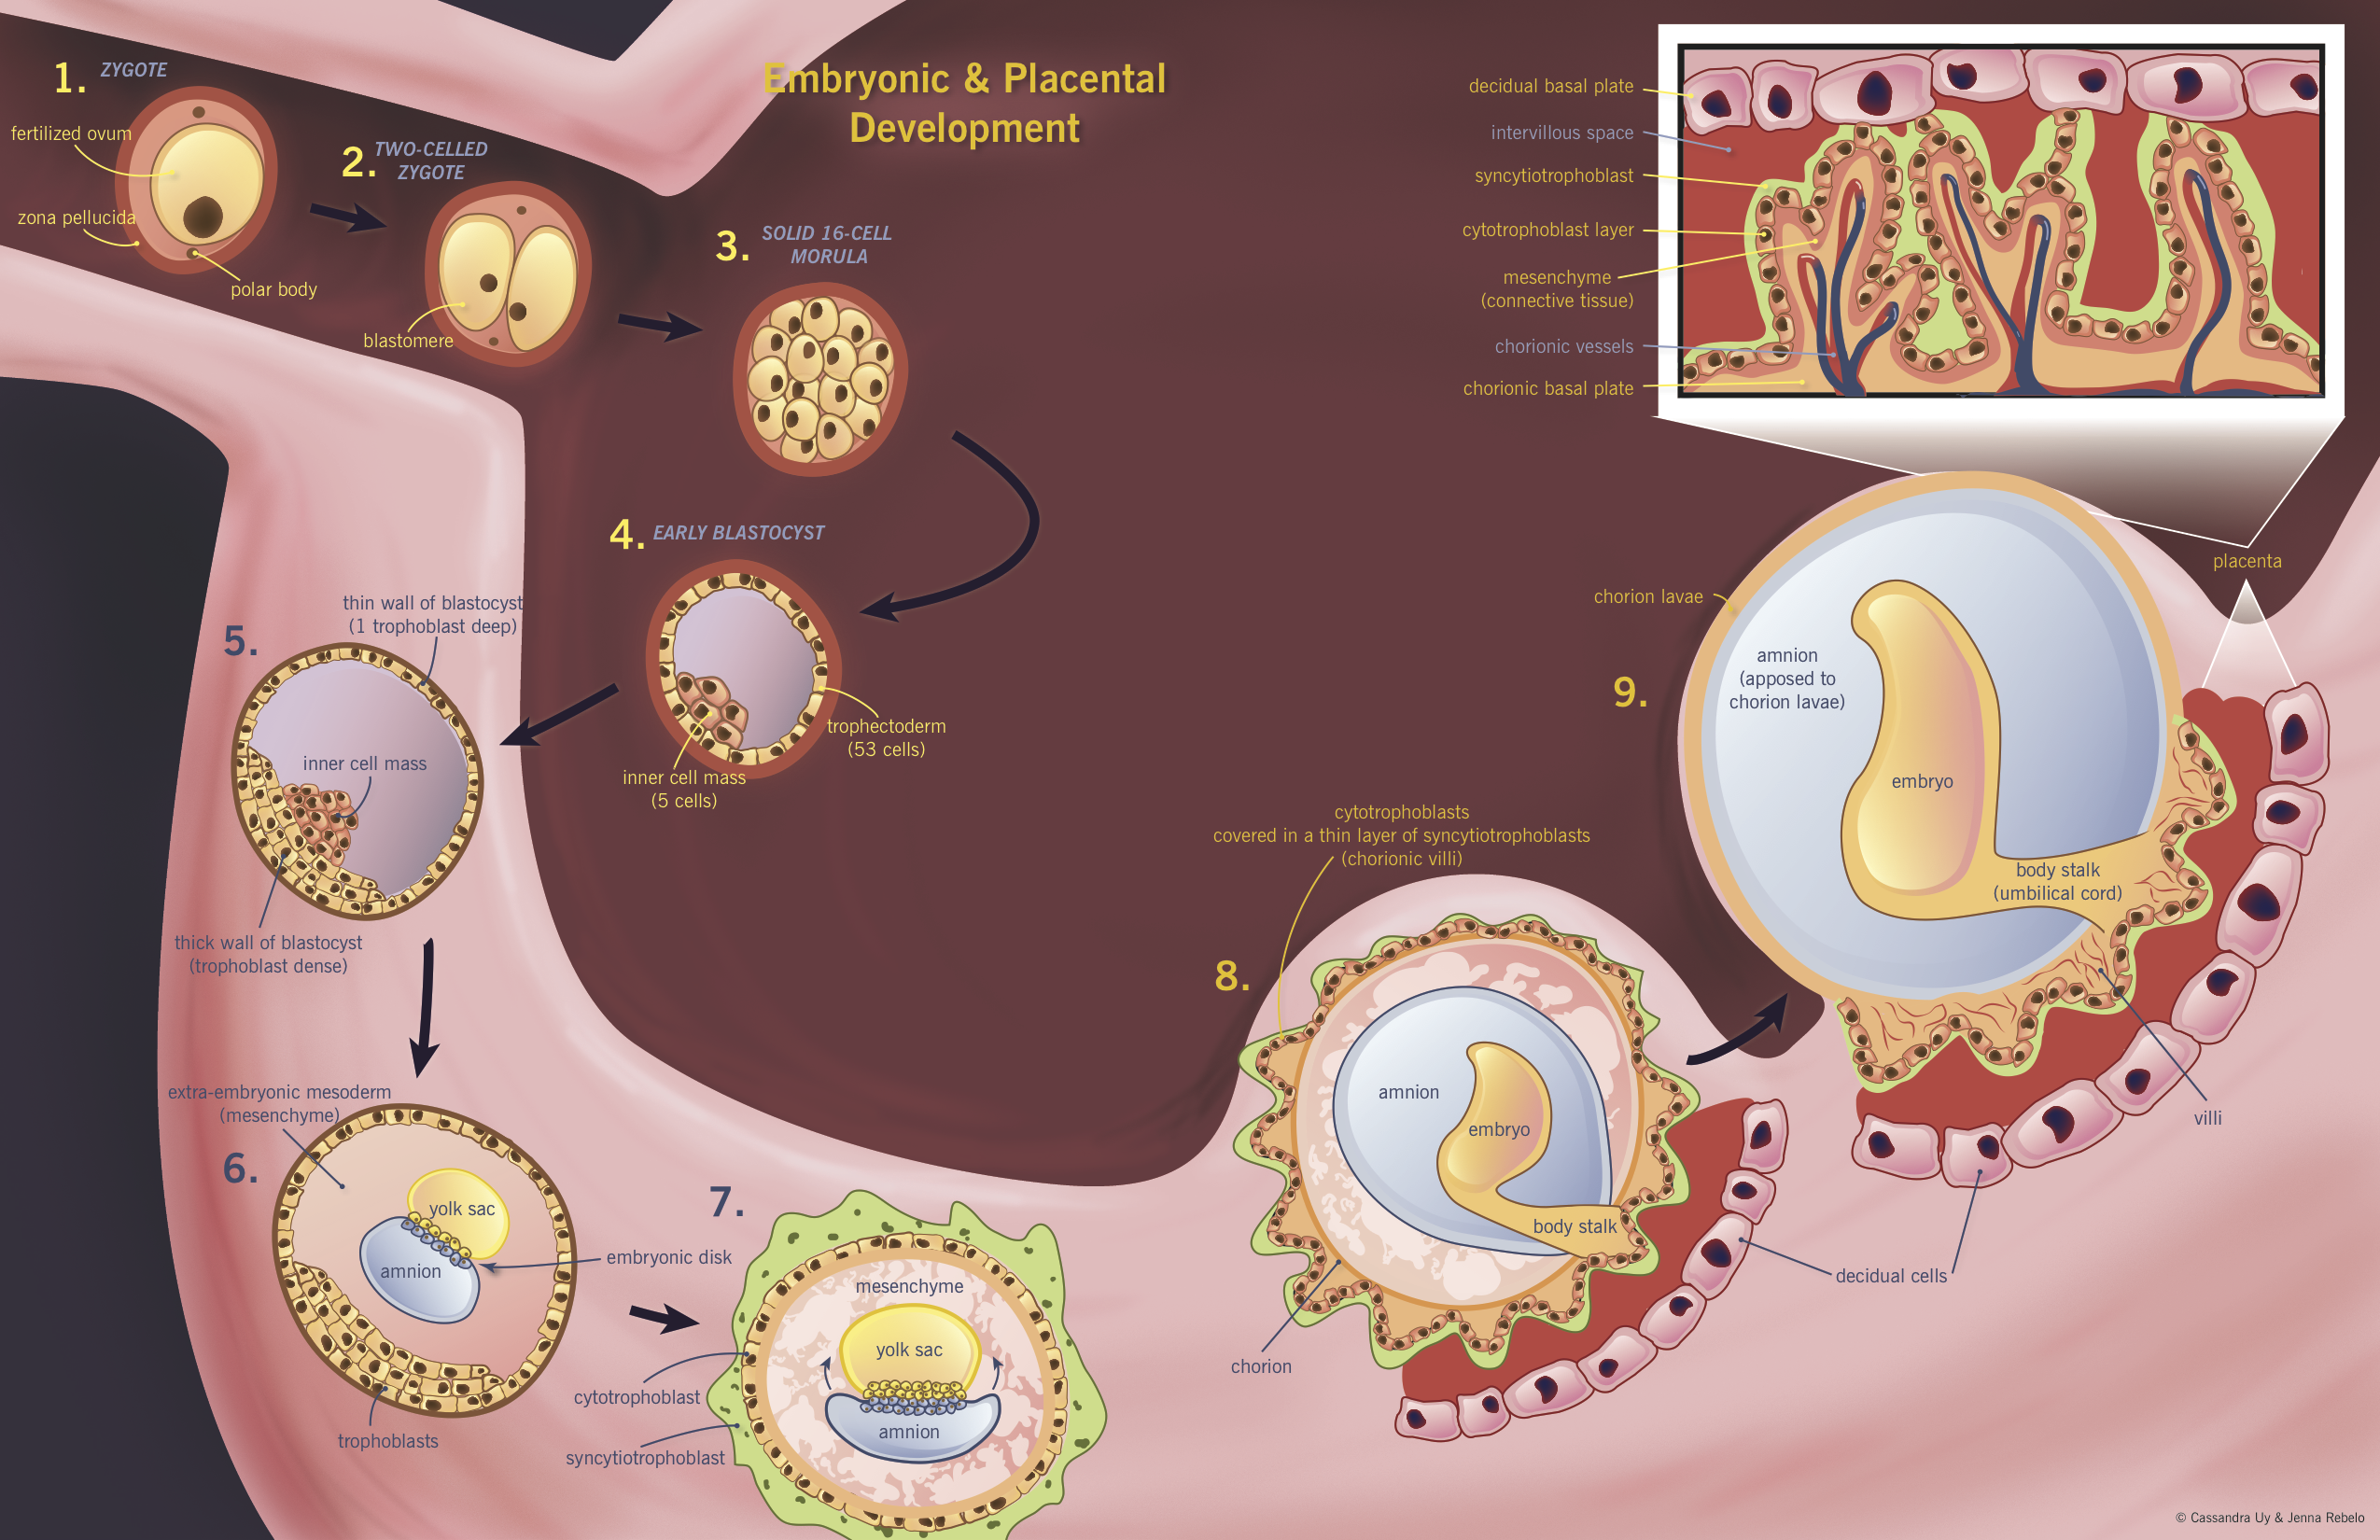
\includegraphics[width=\textwidth,height=6cm]{implantation.png}
    \end{figure}}
\end{itemize}
\end{frame}
%------------------------------------------------------
\begin{frame}{Early Development}
Support System
\begin{itemize}
    \item Amniotic Sac: a transparent, fluid- filled membrane that surrounds and protects the fetus
    \item Placenta: a support organ for the fetus; it keeps the circulatory systems of the fetus and mother separate, but
    as a semipermeable membrane permits the exchange of some materials between them (oxygen and nutrients from mother to fetus and carbon dioxide and waste products from fetus to mother)
    \item Umbilical cord: a tube containing the blood vessels connecting the fetus and placenta
\end{itemize}
\end{frame}
%------------------------------------------------------
\begin{frame}{Early Development}
Support System
\begin{figure}
    \centering
    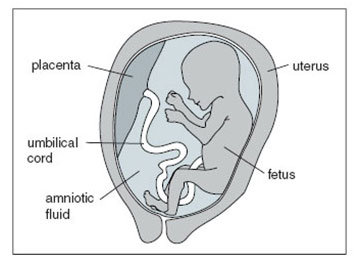
\includegraphics[width=\textwidth,height=6cm]{amniotickey.jpg}
\end{figure}
\end{frame}
%------------------------------------------------------
\begin{frame}{Early Development}
\begin{itemize}
    \item Brain and Spine
    \\ https://www.youtube.com/watch?v=lGLexQR9xGs
    \\ https://www.youtube.com/watch?v=vvBBFOu9h1w
    \begin{figure}
        \centering
        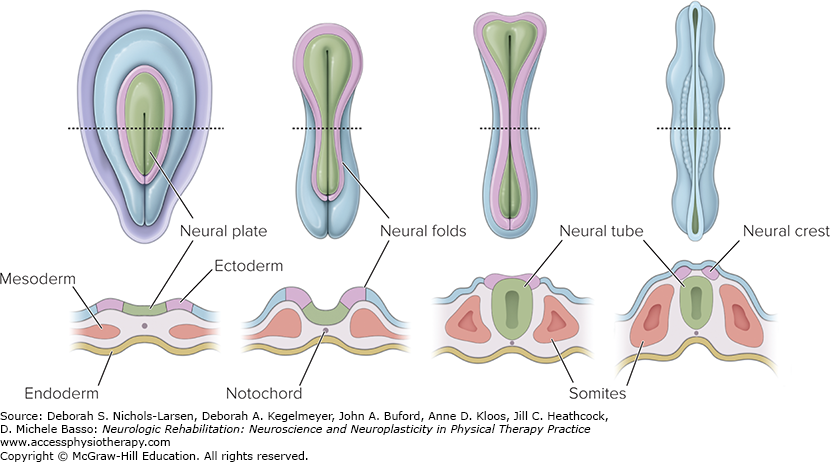
\includegraphics[width=\linewidth,height=4cm]{larsen_ch18_fig-18-04.png}
    \end{figure}
\end{itemize}
\end{frame}
%------------------------------------------------------
\begin{frame}{Early Development}
General Tendency: \textbf{cephalocaudal development} (head first, hand/foot last)
\begin{itemize}
    \item 4 weeks:
    \begin{enumerate}
        \item face begins to emerge
        \item heart is visible and functioning
        \item arm bud visible, leg bud less distinct
    \end{enumerate} 
    \pause
    \item 5.5 week - 8.5 week:
    \begin{enumerate}
        \item 5.5 week: nose, mouth and palate start to differentiate
        \item 8.5 week: nose and mouth fully formed
        \item Cleft Palate
    \end{enumerate}
\end{itemize}
\end{frame}
%------------------------------------------------------
\begin{frame}{Early Development}
\textbf{Cleft Palate}
\begin{figure}
    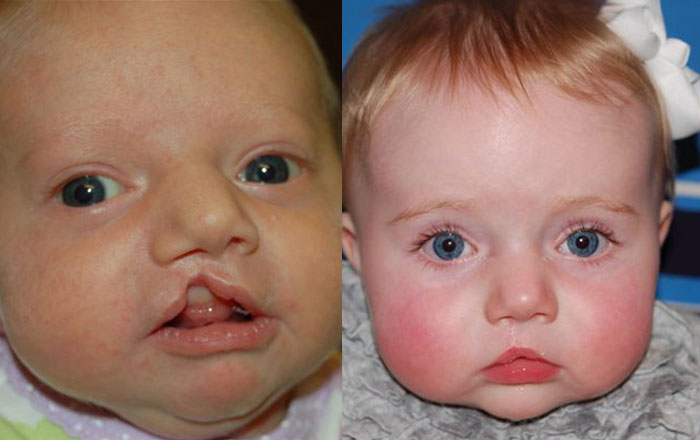
\includegraphics[width=0.457\linewidth,height=6cm]{culley-before-after.jpg}
    \hfill
    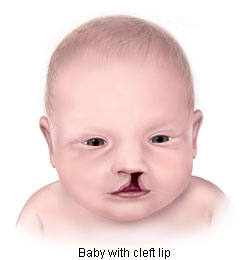
\includegraphics[width=0.457\linewidth,height=6cm]{cleftlip_small.jpg}
\end{figure}
\end{frame}
%------------------------------------------------------
\begin{frame}{Early Development}
\begin{itemize}
    \item 9 week:
    \begin{enumerate}
        \item Eyes and ears are forming
        \item Internal organs are present
        \item Sexual Differentiation
        \item Ribs, fingers, toes, nails are growing
    \end{enumerate}
    \pause
    \item 11 week:
    \begin{enumerate}
        \item Adult-structured heart
        \item Developing spine and major divisions of brain
    \end{enumerate}
\end{itemize}

\end{frame}
%------------------------------------------------------
\begin{frame}{Early Development}
\begin{itemize}
    \item 16 week
    \begin{enumerate}
        \item Kicks
        \item External Genitalia developed (Gender Reveal)
        \end{enumerate}
    \pause
    \item 18 week
    \begin{enumerate}
        \item Sucking thumb
    \end{enumerate}
    \pause
    \item 20 week
    \begin{enumerate}
        \item Facial expressions present
        \item Weight gain -- less movement
    \end{enumerate}
    \pause
     \item 28 week
    \begin{enumerate}
        \item Brain and lungs are sufficiently developed (survive on premature birth)
        \item Rapid eye movement (REM) sleep
        \item Auditory system functioning
    \end{enumerate}
\end{itemize}
\end{frame}
%------------------------------------------------------
\begin{frame}{Fetal Behavior}
\begin{itemize}
    \item Swallowing
    \begin{enumerate}
        \item Swallow amniotic fluid
        \item Promotes palate development (Walker & Quarles, 1976)
        \item Helps digestive system to mature
    \end{enumerate}
    \pause
    \item Breathing
    \begin{enumerate}
        \item Chest movement (in and out)
        \item No air taken in, but small amout of amniotic fluid
    \end{enumerate}
\end{itemize}
\end{frame}
%------------------------------------------------------
\begin{frame}{Fetal Experience}
\begin{itemize}
    \item Touch
    \begin{enumerate}
        \item Sensitive to tactile
        \item Mouth and hand interaction
        \item Bumps into uterus wall 
    \end{enumerate}
    \pause
    \item Taste
    \begin{enumerate}
        \item Differentiating taste of amniotic fluid
        \item Fetuses prefer sweetened amniotic fluid 
    \end{enumerate}
    \pause
    \item Smell
    \begin{enumerate}
        \item Fetuses can detect odors in amniotic fluid
        \item Amniotic fluid can have various odors
    \end{enumerate}
    \pause
    \item Hearing
    \begin{enumerate}
        \item Fetuses responds to sounds as early as 6 month pregnancy
        \item External sounds can change fetal movements and heart rates
        \item Important for speech and language development
    \end{enumerate}
\end{itemize}
\end{frame}




\end{document}